Una de las formas más completas de medir el desarrollo del proyecto es mediante
diagramas de Gantt. Estos diagramas muestran una evolución en el tiempo de
las distintas tareas que conforman el proyecto dividiéndolas en \textit{milestones},
fases y tareas.

En particular, se van a presentar dos diagramas: el primero que muestra el
planteamiento inicial de las fases del proyecto (figura \ref{fig:gantt-original})
y un segundo que muestra el desarrollo real del mismo (figura \ref{fig:gantt-real}).

\begin{figure}[H]
  \centering
  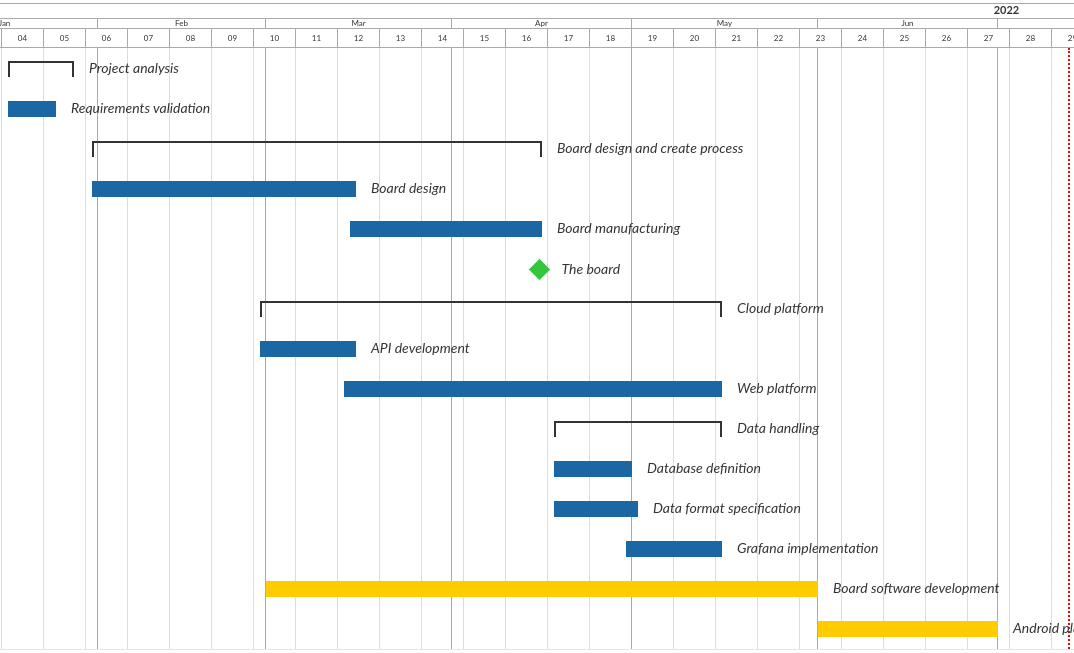
\includegraphics[width=\linewidth]{images/gantt-chart-original.png}
  \caption{Diagrama de Gantt del planteamiento inicial del proyecto.}
  \label{fig:gantt-original}
\end{figure}

De la figura \ref{fig:gantt-original} se pueden extraer las siguientes fases de
desarrollo del proyecto:

\begin{enumerate}
  \item \textbf{Fase de análisis}, en donde se validarían los requisitos del
        proyecto.
  \item \textbf{Fase de diseño}, en donde se diseñaría la placa así como su
        especificación.
  \item \textbf{Fase de implementación}, en donde se realizaría la implementación
        del código fuente de \ac{VIMS} así como de la infraestructura en la nube.
\end{enumerate}

En la primera fase se validaría el documento de requisitos junto con el tutor y
compañeros que se ofreciesen voluntarios a ello (el documento se escribió en julio
de 2021, en lo que habría sido la primera entrega del TFM). Por otra parte, en esta
fase se desarrollarían distintos esquemas que ayudasen a la comprensión de los
requisitos y a la futura implementación del producto.

La segunda fase consistiría en el diseño y desarrollo de la placa que conformaría
el dispositivo \ac{VIMS}. Durante esa fase se detallarían los requisitos técnicos
que necesitaría cumplir la placa para estar conforme a los requisitos previamente
desarrollados. También se incluye en esta etapa el proceso de manufacturación
de la misma.

Mientras tanto, durante las últimas etapas del desarrollo de la placa, se empezaría
a trabajar activamente tanto en la plataforma en la nube como en el código fuente que
ejecutaría la propia placa. El primer paso sería definir la \ac{API} que serviría para
interactuar con la plataforma. A continuación, se definiría la plataforma web y posteriormente
el modelo de datos que se usaría.

Por último, el último mes de desarrollo se dedicaría al desarrollo de la aplicación
Android que serviría de interfaz adicional para el usuario.

\begin{figure}[H]
  \centering
  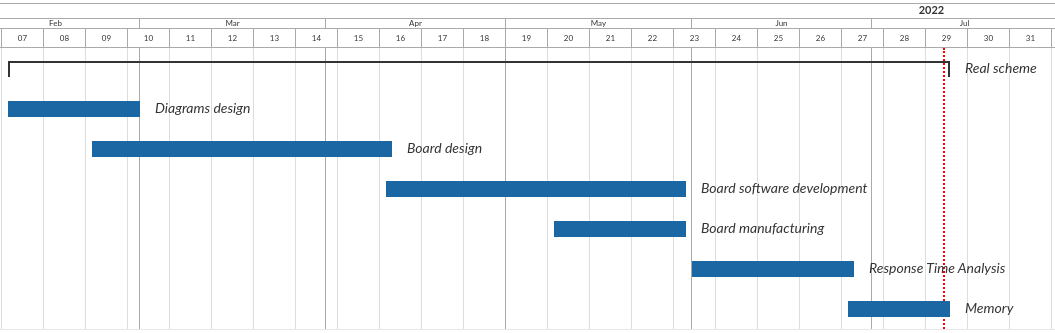
\includegraphics[width=\linewidth]{images/gantt-chart-real.png}
  \caption{Diagram de Gantt final con los tiempos del proyecto.}
  \label{fig:gantt-real}
\end{figure}

Como se puede apreciar en la figura \ref{fig:gantt-real}, el esquema de tiempo final
varía bastante con el planteado inicialmente. Se comentará en más detalle el porqué
en el apartado \ref{sec:drawbacks}. El proyecto al final se planteó como un proyecto
de especificación, sin llegar a realizar una implementación final de un dispositivo,
pese a que se contaba con parte de los materiales (como las placas y las PCBs).

Es por esto que se focalizó gran parte del esfuerzo en el diseño de la placa así como
en los diagramas que modelan el sistema, con la intención de dejarlo lo más
completo posible.

Se empezó a desarrollar el código fuente que ejecutaría el dispositivo \ac{VIMS}
y se realizaron pruebas de diversa índole, todas ellas con éxito:

\begin{itemize}
  \item Se probó que el dispositivo \ac{VIMS} era capaz de recibir su ubicación
        usando \ac{GPS}.
  \item Se probó que el dispositivo \ac{VIMS} podía conectarse a Internet mediante
        el uso de redes WiFi.
  \item Se probó que el dispositivo \ac{VIMS} podía emparejarse a otro dispositivo
        mediante Bluetooth.
  \item Se probó que el dispositivo \ac{VIMS} podía emitir mensajes a los dispositivos
        cercanos mediante \ac{BLE}.
  \item Se probó que el dispositivo \ac{VIMS} podía conectarse a Internet mediante
        redes \ac{LTE} con tarjeta SIM.
  \item Se probó que el dispositivo \ac{VIMS} podía almacenar datos en una tarjeta
        microSD.
  \item Se probó que el dispositivo \ac{VIMS} soportaba planificación de tareas
        usando FreeRTOS junto con el \textit{framework} de Arduino.
\end{itemize}

Por otra parte, el código fuente que se comenzó a implementar era el que se conectaba
mediante \ac{OBD}--II al vehículo.

Se observó la complejidad del proyecto a nivel de planificación ya que cuenta con
una gran cantidad de componentes y tareas que deben ejecutarse de forma sincronizada
para asegurarse un correcto funcionamiento del dispositivo. Por ende, a principios
de junio se empezó a trabajar activamente en el análisis del tiempo de respuesta
del proyecto, planteando valores adecuados para los tiempos de cómputo, tiempo
de acceso a recursos, etc. Se fue trabajando en ello hasta obtener el modelo que
se ha presentado en este proyecto.

Por último, en estas últimas dos semanas se ha trabajado activamente en la memoria
del proyecto, en aunar y recoger todas las ideas clave sobre el desarrollo del mismo
con la intención de que sirva de base para continuar con el desarrollo, una vez
se presente esta parte.
